\chapter{Forschungsziel- und Design}

In diesem Kapitel werden das Ziel und der Zweck dieser Arbeit beschrieben, die daraus abgeleiteten Forschungsfragen erläutert und in einen Zusammenhang gestellt. Des Weiteren wird das Vorgehen zur Beantwortung der Forschungsfragen beschrieben. Das Forschungsdesign ist gegliedert in eine Literaturrecherche, die Strukturierung der extrahierten Ergebnisse und die Anwendung des aus den Ergebnissen entstandenen Leitfadens.

\section{Zieldefinition}

\section{Personas}
1) What are the relevant target groups G, e.g., engineers, end users, or lawyers, and which traits characterize each group’s representatives R, e.g., specific background knowledge or cognitive capacities? 2) What are the explananda X, e.g., events or decisions? 3) Which aspects Y of the explananda X must be explained to which target group G, e.g., why is a decision justified, which causal chain of internal system events led up to it, why did some event e happen instead of event e 4) In which context C may an aspect Y need explanation, and what are the implied constraints? For example, explanations might have to be aural in a driving situation. \cite{kohl_explainability_2019} Die genanten Abhängigkeiten müssen beatnwortet werden.


\section{Forschungsfragen}

\begin{figure}[htb!]
    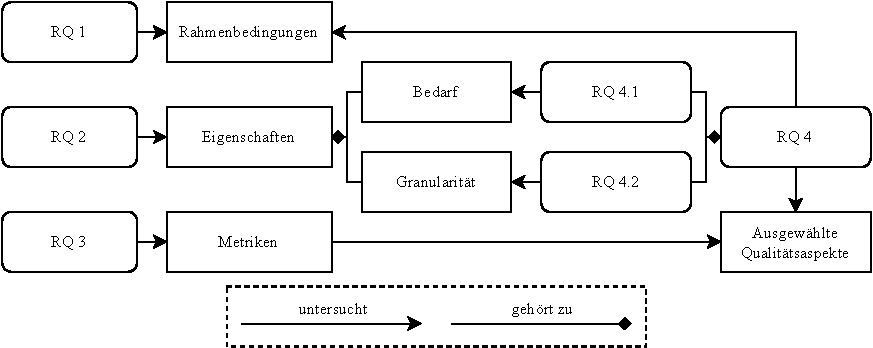
\includegraphics{contents/03_research_design/res/research_questions_overview.pdf}
    \caption{Zusammenhänge der Forschungsfragen}
    \label{fig:research_questions_overview}
\end{figure}

Aus dem Forschungsziel wurden insgesamt fünf Forschungsfragen abgeleitet, welche die Richtung der Arbeit fein granularer definieren. Jede Forschungsfrage behandelt entweder einen konkreten Betrachtungsgegenstand von Erklärbarkeit oder den Zusammenhang dieser einzelnen Aspekte. Wie die einzelnen Forschungsfragen voneinander abhängen, ist in \autoref{fig:research_questions_overview} dargestellt.

\smallskip

\noindent\fbox{
    \parbox{0.965\textwidth}{
        \smallskip
        \textbf{RQ1} Welche Rahmenbedingungen haben einen Einfluss auf die Anforderungen für Erklärungen?
        \smallskip
    }
}

\smallskip

Erklärbare Systeme können sehr verschiedene Ausprägungen haben (z.B. Empfehlungssystem \cite{nunes_systematic_2017} oder Autonome Fahrzeuge \cite{wiegand2019drive}). Auch werden je nach Anwendungsgebiet verschiedene Anforderungen an die Systeme gestellt oder es gibt zusätzlich geltende, äußere Bedingungen \cite{chazette_knowledge_nodate}.

Welche dieser Aspekte einen Einfluss auf die benötigten Erklärungen bzw. Erklärbarkeit im Allgemeinen haben, deckt diese Frage ab. Vor allem konzentriert sich die Frage darauf über welche Rahmenbedingungen sich Stakeholder, die Erklärungen in ein Software-System integrieren möchten, Gedanken machen sollten, um Anforderungen an diese zu formulieren. Dies beinhaltet auch die Ziele, die der Stakeholder für die Software hat.

\smallskip

\noindent\fbox{
    \parbox{0.965\textwidth}{
        \smallskip
        \textbf{RQ2} Welche Eigenschaften von Erklärungen haben einen Einfluss auf die externe Qualität eines erklärbaren Systems?
        \smallskip
    }
}

\smallskip

Es existieren bereits verschiedene Frameworks, welche in bestimmten Kontexten einen Überblick darüber geben, welche Möglichkeiten es gibt, Erklärungen zu gestalten \cite{nunes_systematic_2017}. Vor allem im Bereich der Künstlichen Intelligenz gibt es zahlreiche Arbeiten, welche verschiedene Möglichkeiten vorstellen, um automatisch Erklärungen für komplexe Algorithmen zu generieren \cite{sokol_explainability_2020, mahoney2019framework}.

Um der Forderung nach einem stärkeren Fokus auf den Menschen bei der Betrachtung von Erklärbarkeit nachzukommen \cite{ehsan_operationalizing_2021}, stellt diese Forschungsfrage die externen Qualitätsaspekte \cite{international2011iso} in den Mittelpunkt. Außerdem betrachtet diese Frage die genauen Gestaltungsmöglichkeiten, die Entwicklern oder Designern bei der Konzeption von Erklärungen geboten werden. Folglich ist die Antwort auf diese Frage eine zentrale Grundlage für den Leitfaden, dessen Entwicklung ein Ziel dieser Arbeit ist.

\smallskip

\noindent\fbox{
    \parbox{0.965\textwidth}{
        \smallskip
        \textbf{RQ3} Anhand welcher Metriken kann gemessen werden, ob die in ein erklärbares System integrierten Erklärungen das Ziel der Integration bezogen auf externe Qualitätsaspekte erfüllt haben?
        \smallskip
    }
}

\smallskip

Erklärbarkeit ist eine NFR, welche von vielen verschiedenen Faktoren abhängt und diese auch beeinflusst \cite{chazette_knowledge_nodate}. Die Integration von Erklärungen hat in der Regel Effekte auf mehrere andere Qualitätsaspekte. Diese können sowohl positiv als auch negativ ausfallen. Ein Problem, welches durch die Integration von Erklärungen leicht entstehen kann, ist, dass sich die \textit{Usability} des Systems verschlechtert, wenn sie nicht explizit mitgedacht wird \cite{sokol_explainability_2020}. Folglich stellt das Messen der Qualität von Erklärungen aufgrund der vielfältigen Effekte eine Herausforderung dar. Unterstützt wird dies dadurch, dass viele der durch Erklärbarkeit beeinflussten NFRs vor allem subjektiv von Software-Nutzern wahrgenommen und somit nur wenige objektive Metriken einsetzbar sind \cite{sokol_explainability_2020}.

Zwar wurden in der Literatur bereits Erklärungen anhand verschiedener Metriken analysiert \cite{wiegand2019drive,briand1995goal}. Es fehlt allerdings ein Überblick, welche Metriken zum Messen und zur Bewertung der Qualität von Erklärungen geeignet und erprobt sind. Folglich ist das Ziel bei der Beantwortung dieser offenen Frage, die Metriken, welche bereits zur Evaluation von Erklärungen genutzt wurden, zusammenzutragen.

\smallskip

\noindent\fbox{
    \parbox{0.965\textwidth}{
        \smallskip
        \textbf{RQ4.1} Welchen Einfluss haben der Kontext und die Zielsetzung eines erklärbaren Systems auf den Bedarf für Erklärungen in Bezug auf die externe Qualität des Systems, wenn Erklärungsbedarf besteht?

        \smallskip

        \textbf{RQ4.2} Welchen Einfluss haben der Kontext und die Zielsetzung eines erklärbaren Systems auf die Granularität von Erklärungen in Bezug auf die externe Qualität des Systems, wenn Erklärungsbedarf besteht?
        \smallskip
    }
}

\smallskip

In den ersten drei Forschungsfragen wurden verschiedene Aspekte von Erklärbarkeit behandelt, die wichtig sind, um darauf basierend Erklärungen in ein System zu integrieren. Es fehlt allerdings die Möglichkeit, anhand der Antworten auf diese Fragen eine Auswahl bei der Gestaltung von Erklärungen zu treffen. Eine Antwort auf diese letzten beiden Fragen soll diesen Prozess unterstützen.

Die Einflüsse, nach denen RQ4.1 fragt, sollen bei der Einschätzung helfen, ob und wenn ja, an welchen Stellen ein System Erklärungen benötigt. Dies soll Entwicklern und Designern dabei helfen, die Frage nach dem Bedarf für Erklärungen Anwendungsfall-übergreifend zu beantworten. Für Navigationsanwendungen haben dies beispielsweise \citeauthor{chazette_end-users_nodate} und \citeauthor{wang_integration_2020} bereits getan \cite{chazette_end-users_nodate,wang_integration_2020}.

Wenn eben dieser Bedarf besteht, muss anschließend die Ausgestaltung dieser Erklärung betrachtet werden. Welche bereits untersuchten Einflüsse in Bezug auf diese Granularität von Erklärungen bereits bestehen soll die Antwort auf die Frage RQ4.2 beantworten.

Folglich stellen die Forschungsfragen RQ4.1 und RQ4.2 die Schnittstelle zwischen den ersten drei Forschungsfragen dar.

\bigskip

Die Vorgehensweise dieser Arbeit zum Erreichen des vorgestellten Ziels und bei der Beantwortung der aus dem Ziel abgeleiteten Forschungsfragen wird im folgenden Abschnitt vorgestellt.

\section{Forschungsdesign}
\begin{figure}[htb!]
    \begin{center}
        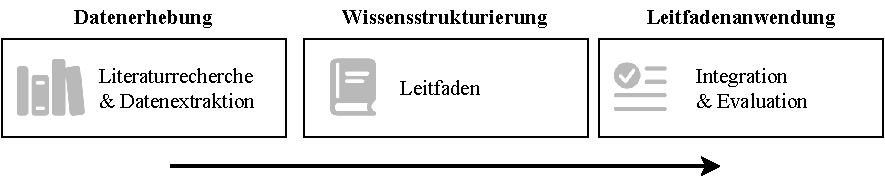
\includegraphics[width=\textwidth]{contents/03_research_design/res/research_design_overview.pdf}
    \end{center}
    \caption{Überblick des Forschungsdesigns}
    \label{fig:research_design_overview}
\end{figure}

Eine Übersicht der Vorgehensweise zur Beantwortung der Forschungsfragen ist in \autoref{fig:research_design_overview} dargestellt. Der Forschungsansatz besteht aus zwei wesentlichen zusammenhängenden Teilen.

Zunächst wurden Daten zum aktuellen Wissensstand über die Aspekte von Erklärungen sowie dessen Zusammenhänge und Auswirkungen auf Softwarequalität erhoben. Zu diesem Zweck wurde eine Literaturrecherche mittels der Suchstring-Methode \cite{kitchenham2004procedures} durchgeführt. Die Antworten auf die Forschungsfragen sind aus den selektierten Arbeiten extrahiert worden, wobei zunächst die Forschungsfragen RQ1 bis RQ3 bearbeitet wurden, um darauf aufbauend die Fragen nach den Einflüssen (RQ4.1 und RQ4.2) zu beantworten.

Auf Basis der Resultate dieser Datenerhebung konnten die Ergebnisse zu den ersten drei Forschungsfragen in ein Modell über die Aspekte von Erklärbarkeit überführt werden. Dies orientiert sich sowohl an Strukturen, welche die Literaturrecherche ergeben hat, als auch an den Forschungsfragen und der Definition von Erklärbarkeit von \citeauthor{chazette_knowledge_nodate} \cite{chazette_knowledge_nodate} (siehe \autoref{sec:model_explanation_aspects}).

Die erhobenen Daten zur Beantwortung der Forschungsfragen RQ4.1 und RQ4.2 sind in einem Katalog der Zusammenhänge zwischen Rahmenbedingen, Charakteristiken von Erklärungen und dem Einfluss auf ausgewählte für Endnutzer wahrnehmbare  Qualitätsaspekte (externe Qualitätsaspekte) gebündelt. Als Schlussfolgerung daraus wurden zusätzlich Design-Empfehlungen abgeleitet.

\bigbreak

Der zweite Teil der Forschung besteht aus der Anwendung des entstandenen Leitfadens. Dies dient der Prüfung, ob der Leitfaden die Integration von Erklärungen in ein bestehendes System unterstützt. Das Ziel ist es, durch neu integrierte Erklärungen positive Auswirkungen auf zuvor definierte Qualitätsziele zu erhalten.

Die Prüfung der Praxistauglichkeit des Leitfadens wurde zusammen mit dem Unternehmen \textit{Graphmasters GmbH} \footnote{\url{https://www.graphmasters.net}, besucht: 10.09.21} aus Hannover durchgeführt. \textit{Graphmasters} ist unter anderem das entwickelnde Unternehmen hinter der Navigationssoftware \textit{NUNAV Navigation} \footnote{\url{https://www.nunav.net}, besucht: 10.09.21}, welches ein Smartphone-Navigationssystem für Endnutzer mit einem kollaborativen Routing-Ansatz ist (Für mehr Details siehe \autoref{sec:model_evaluation}).

Zunächst wurden bestehende Nutzungsprobleme von \textit{NUNAV} analysiert. Darauf basierend hat ein interdisziplinäres Team von \textit{Graphmasters} in einem vorbereiteten Workshop (siehe \autoref{sec:appendix_workshop_protocol}) anhand des zuvor entwickelten Leitfadens grundlegende Ideen für Erklärungen gesammelt. Mithilfe dieser konnten konkrete Anforderungen abgeleitet werden.

Auf Basis der Ergebnisse wurden dann mehrere Erklärungstypen entwickelt und in NUNAV integriert. Diese sind im nächsten Schritt in einer \textit{Case Study} mit Nutzern des Systems evaluiert worden.

Als Abschluss der Forschung wurde zur besseren Interpretation der qualitativen Ergebnisse der \textit{Case Study} ein nicht repräsentatives qualitatives Experiment (Quasi-Experiment) unter Nutzern von \textit{NUNAV Navigation} durchgeführt.

\bigskip

In den folgenden Kapiteln werden die einzelnen beschriebenen Schritte zusammen mit den Ergebnissen näher erläutert.